\chapter{Riconcilazione sorgenti}

Nel seguito verranno documentati i passi intrapresi nella progettazione
del modello riconciliato o Operational Data Store partendo dalle sorgenti
operazionali descritte nel capitolo precedente.

\section{Ispezione e normalizzazione}

\subsection{Helbiz}

Il livello di granularità delle profilazioni della sorgente Helbiz è
risultato essere troppo basso rispetto alle interrogazioni a cui il data
warehouse si prefigge di rispondere. Inoltre attributi come
\textit{latitude}, \textit{longitude}, \textit{battery\_level\_miles},
\textit{power} e \textit{miles\_range} appaiono lontani dal poter
essere inseriti in un costrutto di selezione applicato da un
applicativo che effettua interrogazioni OLAP. Inoltre gli attributi
\textit{battery\_level\_miles} e \textit{miles} risultano essere
ridondanti.

Partendo dallo schema ER mostrato in figura~\ref{fig:vehicle_profiling_er} è
stato ricavato lo schema concettuale di figura
\ref{fig:vehicle_interval_profiling_er}.

\begin{figure}[H]                                                                                                                                                            
\centering                                                                                                                                                                   
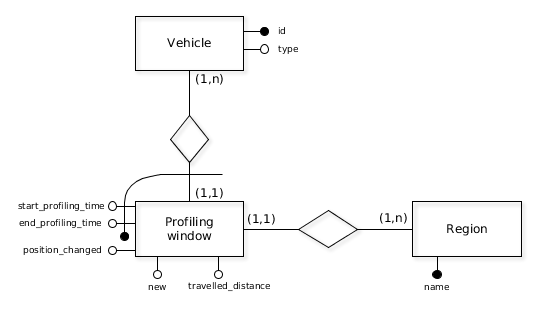
\includegraphics{diagrams/vehicle_interval_profiling_er}                                                                                                                                   
\caption{Diagramma ER Vehicle-Profiling window-Region}                                                                                                                                            
\label{fig:vehicle_interval_profiling_er}                                                                                                                                                           
\end{figure}

Non essendo il nuovo schema una semplice ristrutturazione dello
schema logico di partenza ma un nuovo schema a se stante, l'entità
\textit{Profiling} è stata sostituita con l'entità \textit{Profiling
window}, le cui istanze si riferiscono ai dati profilati all'interno di
un delimitato intervallo di tempo per un determinato veicolo.
Nello specifico sono stati aggiunti i seguenti nuovi attirbuti:
\begin{itemize}
\item \textit{start\_profiling\_time:} istante di inizio della finestra
temporale;
\item \textit{end\_profiling\_time:} istante di fine della finestra temporale;
\item \textit{position\_changed:} attributo che indica se la posizione
del veicolo è variata durante l'intervallo in oggetto;
\item \textit{new:} attributo che indica se un veicolo non presente durante
all'istante di inizio della finestra temporale è stato invece censito
all'istante che delimita la fine della finestra temporale;
\item \textit{travelled\_distance:} attributo che contiene la distanza 
percorsa dal veicolo nella finestra temporale.
\end{itemize}

L'attributo \textit{travelled\_distance} corrisponde alla distanza in linea
d'aria tra le coordinate cartesiane della profilazione effettuata all'istante
\textit{start\_profiling\_time} e quella effettuata all'istante
\textit{end\_profiling\_time}.
L'aggiunta dell'attributo \textit{new} è volta a gestire il caso in cui un
veicolo sia stato oggetto di utilizzo ininterrotto da parte di un utente per
un tempo superiore all'intervallo tra due successive profilazioni o il caso in
cui un veicolo sia stato intenzionalmente posizionato in un punto da un addetto
della manutenzione di Helbiz dopo essere stato ricaricato o allo scopo di
redistribuzione della flotta di veicoli a disposizione.
L'attributo \textit{psotion\_changed} è stato aggiunto allo scopo di permettere
una veloce selezione delle istanze dell'entitò in oggetto per le quali lo
spostamento memorizzato nell'attributo \textit{travelled\_distance} risulta essere
sopra una certa soglia. Come sarà descritto nella parte dedicata alle attività di
ETL eseguite dalle sorgenti operazionali all'ODS, tale attributo permette di
escludere una serie di falsi positivi dati dalla presenza dei veicoli in ambienti
aperti, soggetti agli eventi atmosferici oltre che all'interazione con attori
che si trovano nelle immediate vicinanze.

